\documentclass[10pt, letterpaper ]{article}
\usepackage[ top=2.5cm, bottom=2.5cm]{geometry}

\usepackage{booktabs}
\usepackage{setspace}
\usepackage{graphicx}
\usepackage{hyperref}
\usepackage{graphicx}
\usepackage{caption}
\usepackage{subcaption}
\usepackage{float}
\usepackage{todonotes}
\usepackage{lipsum} % for testing
\usepackage{dsfont}
\usepackage{amsmath}
\usepackage{fixltx2e}
\usepackage{ifluatex}
\usepackage{ifxetex}
\usepackage{parameters/parameters} % own macros created in R file

% allows for compiling with lualatex /xelatex or pdflatex
\ifluatex
  \usepackage{fontspec}
  \setmainfont[ ]{lato}
\else
  \ifxetex
    \usepackage{fontspec}
    \setmainfont[ ]{lato}

  \else
    \usepackage[T1]{fontenc}
    % other font setup
  \fi
\fi



\title{Comparison of Supervised Models \\ Boston Housing Data Set}
\author{Alejandro Kantor}
\date{}

\begin{document} 

\maketitle

\section{Purpose}


Choosing a supervised model for a particular data set depends on several considerations; one of the most important ones is the goodness of fit or performance of the model. In order to facilitate comparing the performance of models for data sets with strictly positive target value and predetermined explanatory variables, we present the program \emph{makeBenchmarking.R} with its corresponding and \LaTeX{} document \emph{documentation.tex}. The R program builds the models detailed in Table~\ref{ta:models} and calculates performance statistics, passing them to objects \LaTeX{} can input. 

As an example, we run the program on the Boston data set which is described in \\ \url{https://archive.ics.uci.edu/ml/datasets/Housing}. 

\begin{table}[h]
	\small
	\centering
	\begin{tabular}{lp{10cm}}
		\toprule
		Model Short Hand & Description \\
		\midrule
		Linear & Linear model with normal error \\
		Gamma1 & Generalized Linear Model with gamma distribution and link~$\mathrm{inverse}$\\
		Gamma2 & Generalized Linear Model with gamma distribution and link~$\log $\\
		Ctree & Conditional Regression Tree from R package \emph{partykit}  using default parameters \\
		Cforrest & Conditional Regression Tree from R package \emph{partykit} using default parameters with~100 iterations \\
		SMV1 &  Support Vector Machine from R package \emph{e1071} using default parameters  \\
		SMV2 & Support Vector Machine from R package \emph{e1071} using default parameters with~$cost = 5$\\
		\bottomrule
	\end{tabular}
	\caption{Description of Models}
	\label{ta:models}
\end{table}

\section{Methodology}


In order to compare the performance of each model detailed in Table~\ref{ta:models}, we apply an 8-fold Cross Validation. In particular, we group the original data into 8 groups and then, for each group, we train the model on the remaining 7 groups and test the performance on the selected group. As a result, we have 8 values for each performance measure, which allows for a more robust comparison between the models. 

Performance is measured by a few statistics. Our primary statistic is the Mean Square Difference (MSE) between the estimated and observed values. As a complementary measure, we look at the Proportion of Cases with an Absolute Log Difference (PCALD) between the estimated and observed values up to a certain threshold $k$, for more information see Appendix~\ref{sec:log-change}. 


\section{Results}


We present the results of running the program on the Boston Data Set in two different formats. We show the average performance indicators for the train and test samples in Tables~\ref{ta:sumTrain} and~\ref{ta:sumTest}, respectively. On the other hand, we show the distribution of MSE and  absolute log change of 0.05 for the test samples, in Figures~\ref{fig:mse} and~\ref{fig:prop05}

In general, we observe that all models have lower average performance indicators in the test samples compared to the train samples, suggesting over-fitting in the training sample.

SVM2 has the best performance in the test samples with a distribution of MSE in general lower to other models (see Figure~\ref{fig:mse}), averaging at \sBestModelMSE, as well as a higher distribution of poprchng0.05 (see Figure~\ref{fig:prop05}), averaging at \sBestModelPropFive. It is also important to note that the performance of \sBestModel{} is considerably higher than the next best model \sSecondBestModel{} . For example the MSE in the test sample that is \sBestChangeMSE\% higher in \sSecondBestModel{} compared to \sBestModel{}. We can see how these two models' estimates compare to the observed value for a test sample in Figure~\ref{fig:comparison}.


\input tables/summaryTrain

\input tables/summaryTest

\begin{figure}[H]
\centering
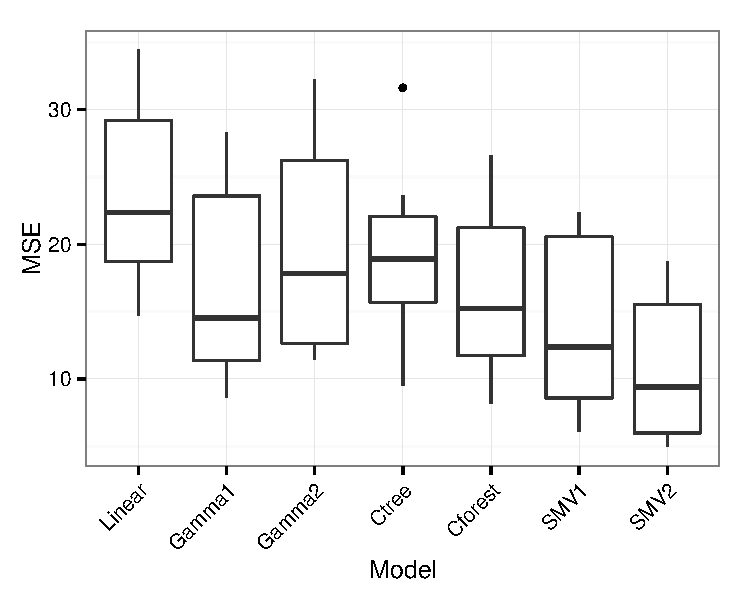
\includegraphics[width=0.7\textwidth]{figures/mse.pdf}
\caption{Distribution of MSE in Test Sample by Model }
\label{fig:mse}
\end{figure}


\begin{figure}[H]
\centering
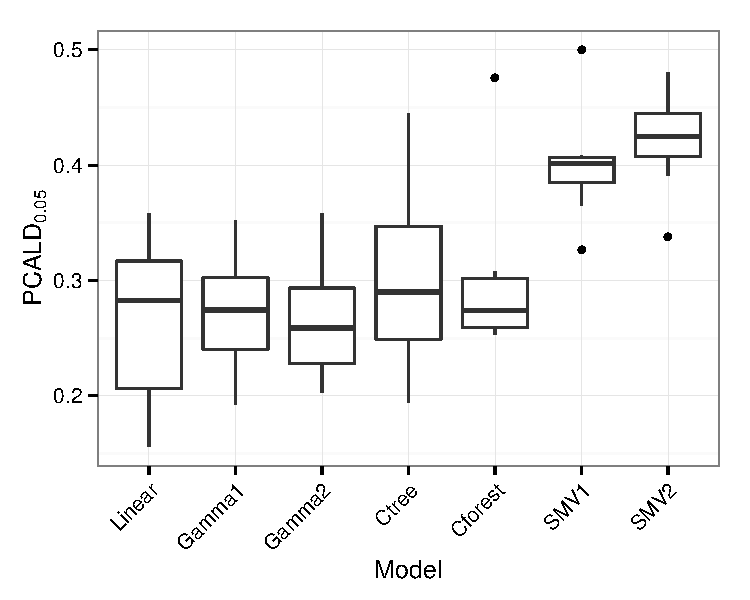
\includegraphics[width=0.7\textwidth]{figures/prop05.pdf}
\caption{Distribution of PCALD\textsubscript{0.05} in Test Sample by Model}
\label{fig:prop05}
\end{figure}



\begin{figure}[H]
	\centering
	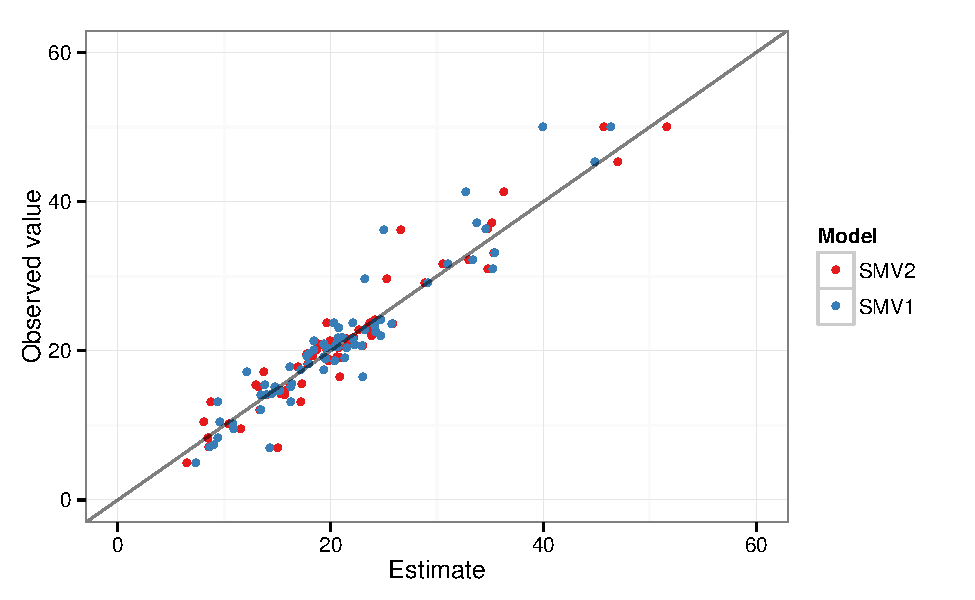
\includegraphics[width=0.8\textwidth]{figures/comparison.pdf}
	\caption{Scatter Plot of Estimates by Models with the Best Performance the Observed Values}
	\label{fig:comparison}
\end{figure}


\section{Conclusions}

The main conclusion of this analysis is that the program successfully allows for the comparison of the performance of the models detailed in Table~\ref{ta:models} with the Boston Housing Data Set. 

We find that the \sBestModel{} model has the best performance followed by the \sSecondBestModel{} model. Thus, if our only consideration is performance, we would suggest using this model for making prediction for the given data set.

%---------------------------------------------------------------

\appendix

\newpage

\noindent{\huge\textbf{Appendix}}

\section{TODOs \& Improvements}

We suggest the following improvements to the program
\begin{itemize} 
\item generalize the process so we can choose which models and performance statistics the program runs and thus allow for classification models and other regression models to be included;
\item modify the code so that Artificial Neural Networks can also be fitted;
\item further modulate the code reducing its repetition; 
\item make a more general latex template for different types of outputs from \emph{makeBenchmarking.R}.
\end{itemize}

\section{Proportion of Cases with Log Difference $\le$ k}
\label{sec:log-change}

The Absolute Log Difference for a give observation $i$ is defined by the following equation.

\begin{equation}
ALD_i = \left\| \log\left(   y_i \right) -\log\left( \hat{y}_i \right) \right\| 
\label{eq:lchange}
\end{equation}

\noindent where $y_i$ is the observed value and $\hat{y}_i$ is the estimated value.

The Proportion of Cases with Log Difference $\le$ k is defined by counting proportion of cases which satisfy $ALD_i \le k$ as shown in the following equation. 

\begin{equation}
PCALD_k = \frac{ \sum_{i=1}^{n} \left( \mathds{1}_{ALD_i \le k} \right)}{ n }
\label{eq:logchange}
\end{equation}

\noindent where $n$ is the number of cases in the data set. 

\section{Scatter Plot Examples}

In this Section, we present the scatter plots of the estimated values by each model with respect to the observed value. This analysis is performed on one of the test samples.

\begin{figure}[H]
	\centering
	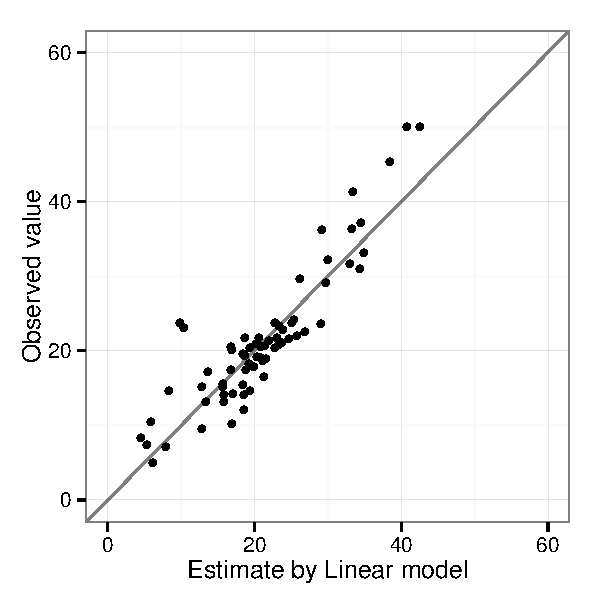
\includegraphics[width=0.49\textwidth]{figures/linear.pdf}
	\caption{Linear}
\end{figure}


\begin{minipage}{0.49\textwidth}
\begin{figure}[H]
	\centering
	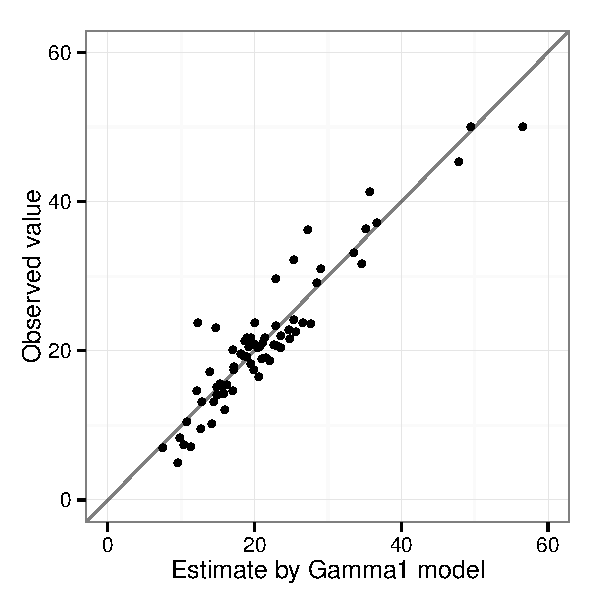
\includegraphics[width=\textwidth]{figures/gamma1.pdf}
	\caption{Gamma1}
\end{figure}
\end{minipage}
\begin{minipage}{0.49\textwidth}
	\begin{figure}[H]
		\centering
	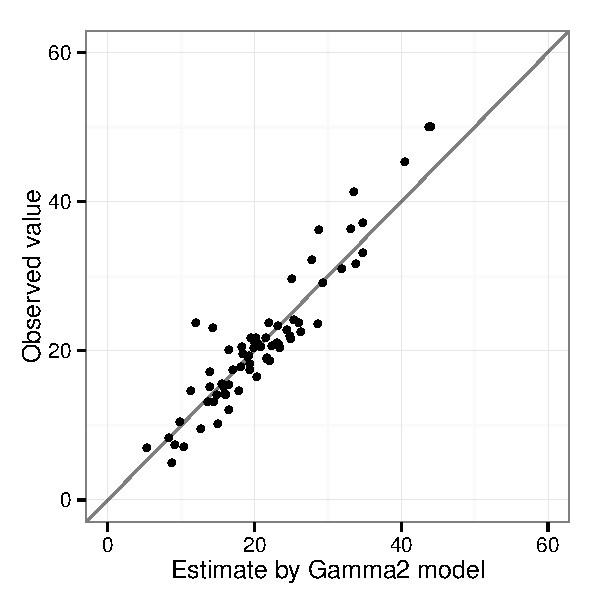
\includegraphics[width=\textwidth]{figures/gamma2.pdf}
	\caption{Gamma2}
	\end{figure}
\end{minipage}

\begin{minipage}{0.49\textwidth}
	\begin{figure}[H]
		\centering
		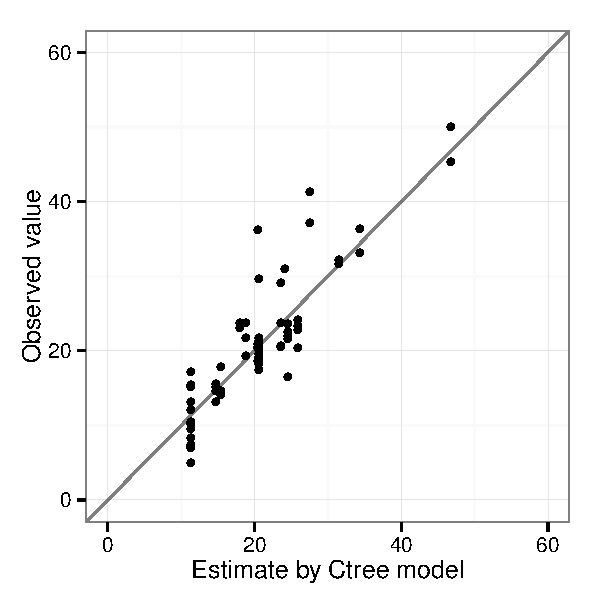
\includegraphics[width=\textwidth]{figures/ctree.pdf}
		\caption{Ctree}
	\end{figure}
\end{minipage}
\begin{minipage}{0.49\textwidth}
	\begin{figure}[H]
		\centering
		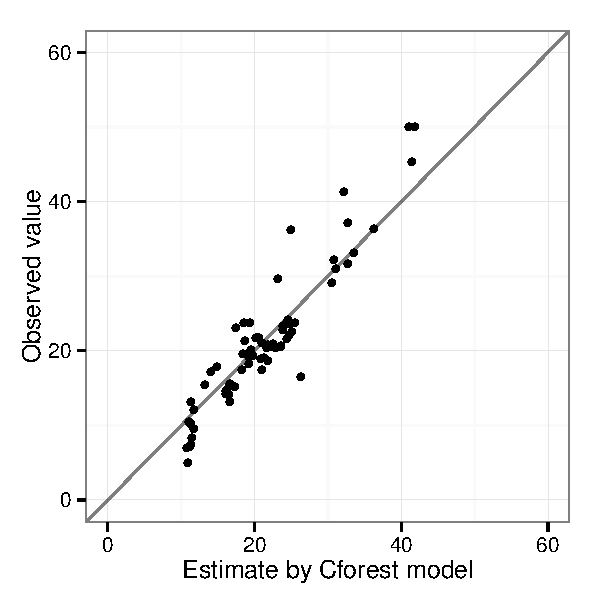
\includegraphics[width=\textwidth]{figures/cforest.pdf}
		\caption{Cforest}
	\end{figure}
\end{minipage}

\begin{minipage}{0.49\textwidth}
	\begin{figure}[H]
		\centering
		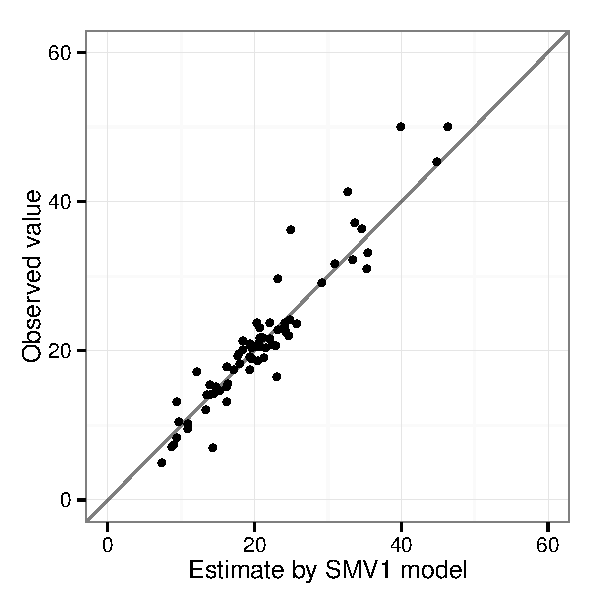
\includegraphics[width=\textwidth]{figures/smv1.pdf}
		\caption{Svm1}
	\end{figure}
\end{minipage}
\begin{minipage}{0.49\textwidth}
	\begin{figure}[H]
		\centering
		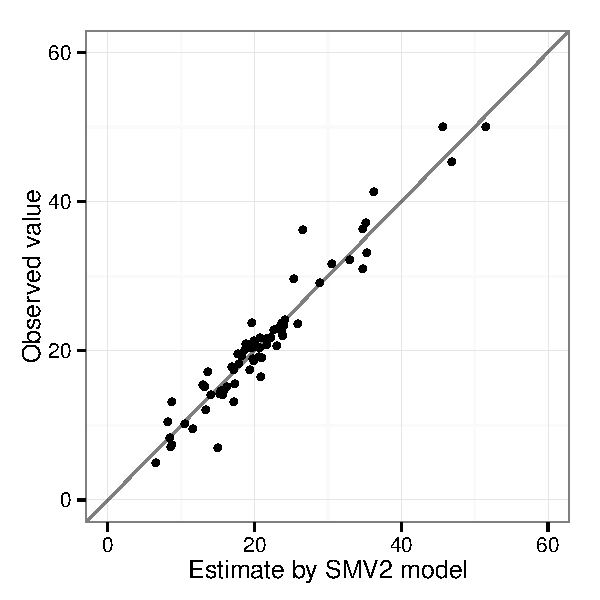
\includegraphics[width=\textwidth]{figures/smv2.pdf}
		\caption{Svm1}
	\end{figure}
\end{minipage}

\end{document}